\section{Background}
\label{sec:background}

Researchers have developed and improved several techniques to model users for 
the past 20 years~\citep{petrelli_user_centered_1999} \citep{fink_adaptable_1997}. 
Modelling users needs to gather knowledge about their capabilities, drawbacks and 
limitations. During these first decades there was not any official and medical-based 
study to consult about user capabilities. Nevertheless, in 2001 this situation 
changed. Under the \ac{who} coordination the World Health Assembly published the
\ac{icf}\footnote{http://www.who.int/classifications/icf/en/} document. 
\ac{icf} is a classification of human functioning and disability. It classifies 
every function state associated with health (e.g., diseases, disruptions, injuries 
and traumas). Its purpose is to identify the low-level capabilities relevant to 
product design in several domains. As was written by experts in the area, the 
\ac{icf} document is a reference for identifying several user capabilities in any 
interaction process. Its goals are the following:

\begin{itemize}
  \item To provide a scientific basis for understanding and studying health and
  health-related states, outcomes and determinants.
  \item To establish a common language for describing health and health-related 
  states in order to improve communication between different users, such as health 
  care workers, researchers, policy-makers and the public, including people with 
  disabilities.
  \item To permit comparison of data across countries, health care disciplines,
  services and time.
  \item To provide a systematic coding scheme for health information systems.
\end{itemize}

It is organized into two main groups: Part 1 deals with \textit{Functioning and
Disability}; Part 2 covers \textit{Contextual Factors}. From the first group the 
following categories are highlighted:

\begin{itemize}
  \item Body functions.
  \item Body structures.
  \item Activities and participation.
  \item Environmental factors.
\end{itemize}

The second group gathers a list of \textit{Environmental Factors} which have an 
impact on all components of functioning and disability.

\ac{icf} considers 8 main components in the context of health:

\begin{description}
  \item[\Defi{Body functions}] \hfill \\
    \begin{mdframed}[hidealllines=true,backgroundcolor=gray!20]
    \textit{``Body functions are the physiological functions of body systems (including
    psychological functions)''.}
    \end{mdframed}
% 
  \item[\Defi{Body structures}] \hfill \\
    \begin{mdframed}[hidealllines=true,backgroundcolor=gray!20]
    \textit{``Body structures are anatomical parts of the body such as organs, 
    limbs and their components''.}
    \end{mdframed}
    
  \item[\Defi{Impairments}] \hfill \\
    \begin{mdframed}[hidealllines=true,backgroundcolor=gray!20]
    \textit{``Impairments are problems in body function or structure such as a 
    significant deviation or loss''.}
    \end{mdframed}

  \item[\Defi{Activity}] \hfill \\
    \begin{mdframed}[hidealllines=true,backgroundcolor=gray!20]
    \textit{``Activity is the execution of a task or action by an individual''.}
    \end{mdframed}

  \item[\Defi{Participation}] \hfill \\
    \begin{mdframed}[hidealllines=true,backgroundcolor=gray!20]
    \textit{``Participation is involvement in a life situation''.}
    \end{mdframed}

  \item[\Defi{Activity limitations}] \hfill \\
    \begin{mdframed}[hidealllines=true,backgroundcolor=gray!20]
    \textit{``Activity limitations are difficulties an individual may have in 
    executing activities''.}
    \end{mdframed} 
    
  \item[\Defi{Participation restrictions}] \hfill \\
    \begin{mdframed}[hidealllines=true,backgroundcolor=gray!20]
    \textit{``Participation restrictions are problems an individual may experience 
    in involvement in life situations''.}
    \end{mdframed}

  \item[\Defi{Environmental factors}] \hfill \\
    \begin{mdframed}[hidealllines=true,backgroundcolor=gray!20]
    \textit{``Environmental factors make up the physical, social and attitudinal
    environment in which people live and conduct their lives''.}
    \end{mdframed} 
\end{description}

\ac{icf} provides a multi-perspective approach to the classification of functioning 
and disability as an \textit{interactive} and \textit{evolutionary} process. It 
provides the building blocks for users who wish to create models and study 
different aspects of this process. The interaction of the components remarked by
\ac{icf} are illustrated in Figure~\ref{fig:icf_interaction}.

\begin{figure}
\centering
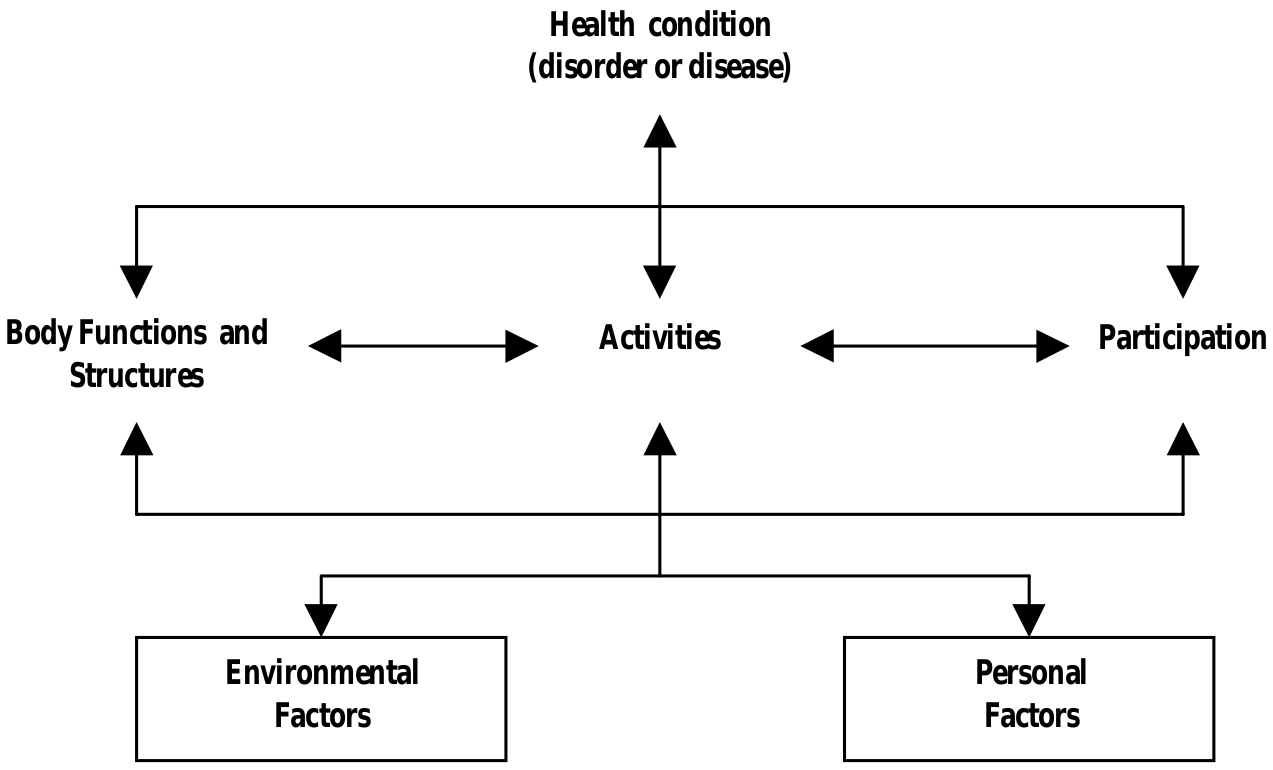
\includegraphics[width=0.75\textwidth]{icf_interaction.png}
\caption{Interactions between the components of~\ac{icf}.}
\label{fig:icf_interaction}
\end{figure}